% (c) Jakub Stejskal
% Master Thesis
% Performance Testing and Analysis of Qpid-Dispatch Router
% Chapter 6

\chapter{Experimental Evaluation}
\label{Experimental Evaluation}
This chapter summarizes results of the performance testing and experimental evaluation of Maestro. We split the experiments into two parts. The first performs a basic measurement of Maestro\,1.3.0 which includes Maestro Agent and AMQP Inspector. During this experiments we focused on reclaiming the highest possible throughput of singlepoint topology of Qpid-dispatch and Message Broker and multipoint topologies with three nodes of Qpid-dispatch and with Broker in the middle. These experimental topologies are depicted in the Figure \ref{fig:basic_topologies}. The later series of experiments are focused on behavior testing of topologies, which involves Qpid-Dispatch reliability and recovery testing.

Since the testing was executed over multiple topology types, we used Topology Generator for quick automatic changes of topology. Each test was executed against established topology where all components were newly installed and restarted between each test scenario. This was done during the cleaning stage. For experimental evaluation we used machines specified in the Table \ref{tab:machines}. The reason why clients use more powerful machines is that we needed more machines for SUT, but only two IBM Xeon machines were available during the experimental evaluation and we needed at least three machines for the SUT nodes. For proper comparison we need all SUTs on the same machine type.

% Please add the following required packages to your document preamble:
% \usepackage[table,xcdraw]{xcolor}
% If you use beamer only pass "xcolor=table" option, i.e. \documentclass[xcolor=table]{beamer}
\begin{table}[H]
\centering
\caption{Machines and their properties, which were used for the experimental evaluation.}
\label{tab:machines}
\begin{tabular}{|l|l|r|r|}
\hline
\rowcolor[HTML]{C5E3DF}
\textbf{} & \multicolumn{1}{c|}{\cellcolor[HTML]{C5E3DF}\textbf{Machine}} & \multicolumn{1}{c|}{\cellcolor[HTML]{C5E3DF}\textbf{CPU}} & \multicolumn{1}{c|}{\cellcolor[HTML]{C5E3DF}\textbf{RAM (Gb)}} \\ \hline
SUT & Opteron & 8 & 8 \\ \hline
Clients & IBM Xeon & 16 & 16 \\ \hline
\end{tabular}
\end{table}

\section{Basic Performance Measurements}
\label{Basic Performance Measurements}
Maestro works as the orchestration system, and requires proper infrastructure before one can run any test for our experimental evaluation. The architecture of Maestro, described in the Chapter \ref{Messaging Performance Tool}, specifies that in ideal scenario one needs at least four machines for running a simple test: maestro broker, sender, receiver, and SUT. The amount of needed machines obviously rises with more complex scenarios and larger networks. Examples of used generated experimental topologies are depicted in the Figures \ref{fig:basic_topologies}. For these configurations we compared the throughput and latency of these combinations. During all measurements we used Maestro Inspector to inspect one of the SUT depending on the topology type. Note, that for Qpid-Dispatch we used AMQP Inspector and for Broker we used ActiveMQ Inspector. The topologies were picked based on current performance testing and known topologies, where some performance degradation was already found during the previous testing.

\begin{figure}[h]
	\centering
	\begin{minipage}{0.45\linewidth}
		\subfloat[Topology with a single router node.\label{fig:basic_topology_router}]{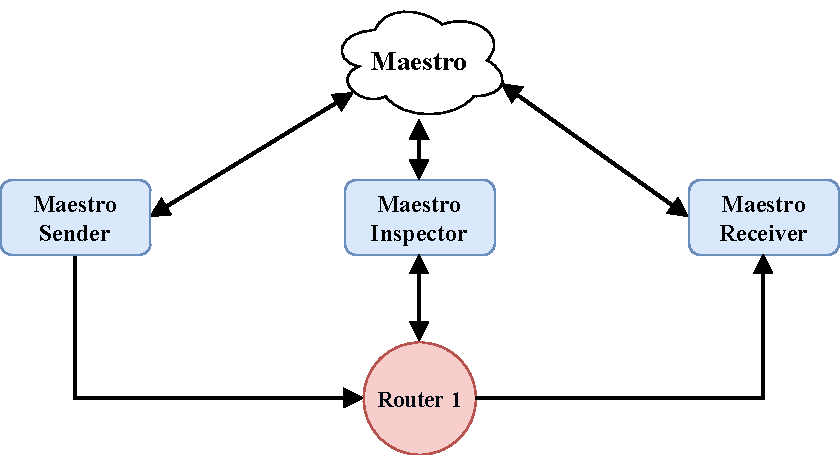
\includegraphics[width=\linewidth]{obrazky-figures/basic_topology_router_single.pdf}}
	\end{minipage}
	\begin{minipage}{0.45\linewidth}
		\subfloat[Topology with a single Broker node.\label{fig:basic_topology_broker}]{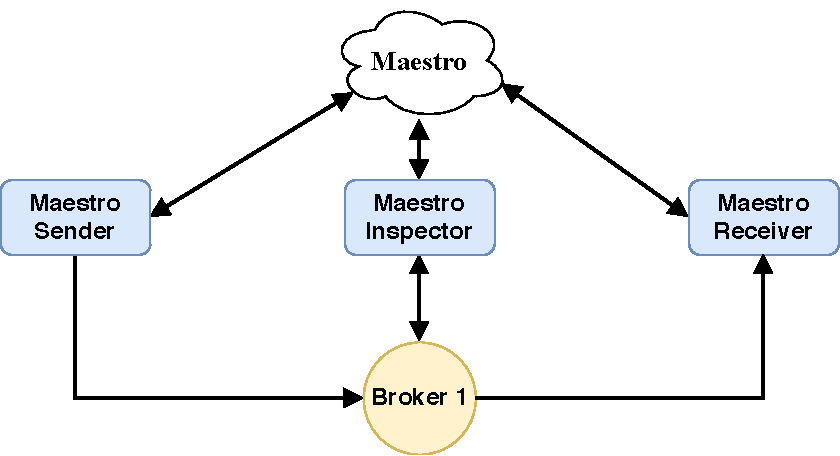
\includegraphics[width=\linewidth]{obrazky-figures/basic_topology_broker_single.pdf}}
	\end{minipage}
	\begin{minipage}{0.45\linewidth}
		\subfloat[Topology consisting of routers nodes only.\label{fig:basic_topology_router_line}]{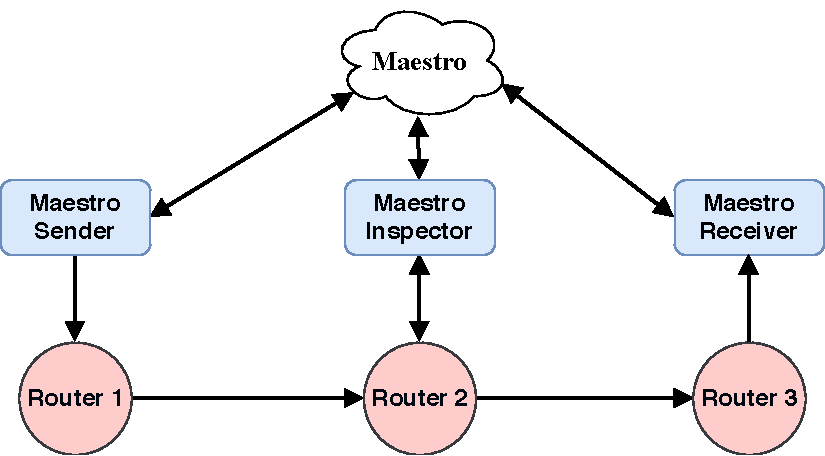
\includegraphics[width=\linewidth]{obrazky-figures/basic_topology_router.pdf}}
	\end{minipage}
	\begin{minipage}{0.45\linewidth}
		\subfloat[Topology with Broker in the middle.\label{fig:basic_topology_broker_line}]{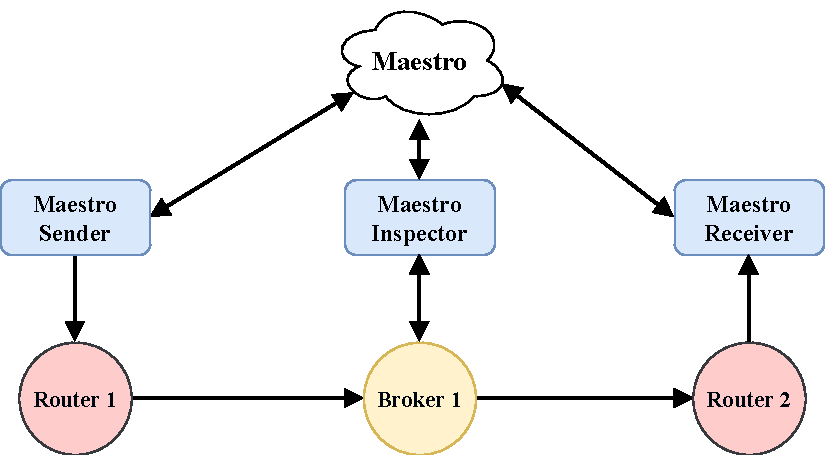
\includegraphics[width=\linewidth]{obrazky-figures/basic_topology_broker.pdf}}
	\end{minipage}
	\caption[Examples of experimental topologies created for basic performance testing and experiments with Maestro.]{Examples of experimental topologies created for basic performance testing and experiments with Maestro. The arrows indicates the communication path between topology components.}\label{fig:basic_topologies}
\end{figure}

Each test case has specific parameters which can be defined by the user. The summary of available parameter is in the following list:
\begin{itemize}
	\setlength\itemsep{0em}
	\item \textbf{MESSAGE\_SIZE}\,---\,message size in bytes.
	\item \textbf{PARALLEL\_COUNT}\,---\,number of connected clients to the SUT during the test.
	\item \textbf{TEST\_DURATION}\,---\,test duration specified as time value (e.g. 120s, 10m) or number of messages (10\,000\,000) to transfer.
	\item \textbf{RATE}\,---\,rate of each connected client; 0 represents unbounded test.
	\item \textbf{INSPECTOR\_NAME}\,---\,name of inspector implementation (ActivemqInspector or InterconnectInspector).
	\item \textbf{MANAGEMENT\_INTERFACE}\,---\,URL where inspector will inspect the SUT.
	\item \textbf{MAESTRO\_BROKER}\,---\,URL to Maestro Broker.
	\item \textbf{SEND\_RECEIVE\_URL} (singlepoint only)\,---\,URL where sender and receiver connects.
	\item \textbf{SEND\_URL}\,---\,URL where sender connects.
	\item \textbf{RECEIVE\_URL}\,---\,URL where receiver connects.
	\item \textbf{EXT\_POINT\_SOURCE}\,---\,URL to public git repository with code handlers.
	\item \textbf{EXT\_POINT\_BRANCH}\,---\,branch which should be used for ext point repository.
	\item \textbf{EXT\_POINT\_COMMAND}\,---\,command executed by the Agent.
\end{itemize}

\subsection{Throughput}
\label{Throughput}
We measured throughput only by load generators\,---\,\emph{Maes\-tro Sender} and \emph{Maestro Receiver}. Load generation depends on the test properties as one can see the test properties for each test case in the Table \ref{tab:test_case_throughput}. Maestro is able to create an unbounded rate test, during which it generates as much load as it can. This type of test was used to reach the maximum handled rate of Qpid-dispatch and Message Broker. The unbound rate during the test is achieved by setting the environment variable \emph{RATE} to value 0. The throughput test cases are focused on maximum throughput of simple or complex topologies.

% Please add the following required packages to your document preamble:
% \usepackage{multirow}
% \usepackage[table,xcdraw]{xcolor}
% If you use beamer only pass "xcolor=table" option, i.e. \documentclass[xcolor=table]{beamer}
\begingroup
\setlength{\tabcolsep}{10pt} % Default value: 6pt
\renewcommand{\arraystretch}{1.35} % Default value: 1
	\begin{table}[H]
	\centering
	\caption{Test case settings for throughput measurements}
	\label{tab:test_case_throughput}
	\begin{tabular}{|l|r|r|r|r|}
	\hline
	\rowcolor[HTML]{C5E3DF}
	\cellcolor[HTML]{C5E3DF}                                         & \multicolumn{4}{c|}{\cellcolor[HTML]{C5E3DF}\textbf{Value}}                                                                          \\ \cline{2-5}
	\rowcolor[HTML]{C5E3DF}
	\cellcolor[HTML]{C5E3DF}                                         & \multicolumn{2}{c|}{\cellcolor[HTML]{C5E3DF}\textbf{Singlepoint}} & \multicolumn{2}{c|}{\cellcolor[HTML]{C5E3DF}\textbf{Multipoint}} \\ \cline{2-5}
	\rowcolor[HTML]{C5E3DF}
	\multirow{-3}{*}{\cellcolor[HTML]{C5E3DF}\textbf{Test Property}} & \textbf{Router}                 & \textbf{Broker}                 & \textbf{Full Router}            & \textbf{With Broker}           \\ \hline
	\textbf{MESSAGE\_SIZE [B]}                          & \multicolumn{4}{r|}{256}                    \\ \hline
	\textbf{PARALLEL\_COUNT}                            & \multicolumn{4}{r|}{5}                      \\ \hline
	\textbf{TEST\_DURATION [m]}                         & \multicolumn{4}{r|}{15m}                    \\ \hline
	\textbf{RATE}                                       & \multicolumn{4}{r|}{0}                   		\\ \hline
	\end{tabular}
	\end{table}
\endgroup



\subsubsection*{Single Node}
The first tests were ran against the single node topologies, which are depicted in the Figures \ref{fig:basic_topology_router} and \ref{fig:basic_topology_broker}. These topologies contains only one SUT node, which is forwarding messages from sender to receiver. During the test the SUT node is inspected by the proper Maestro Inspector.

The measured throughput is depicted in the Figure \ref{fig:rate-single} where one can see the comparison of tests with 15\,minutes duration, which tries to achieve the highest possible throughput. One can see that the maximum throughput of Qpid-Dispatch, as a standalone network component, can reach around 90\,000 messages per second. On the other hand, the lone Messaging Broker reaches only about 30\,000 messages per second. This throughput difference is caused by the fact, that Broker stores all of the messages in the memory until clients want them. This is the main feature of the broker, because it operates as an message distributor in the network. On contrary the router only routes the messages to the destination so it does not need to store message in the memory.

\begin{figure}[H]
	\centering
	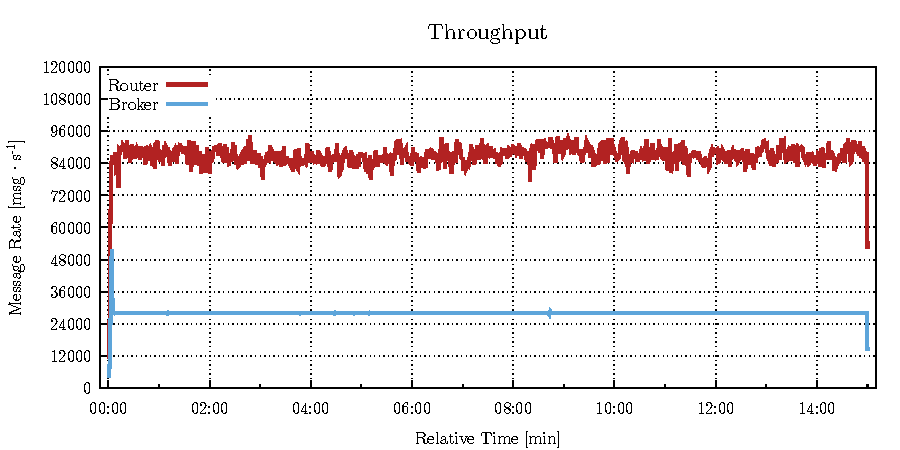
\includegraphics[width=1\linewidth]{obrazky-figures/charts/singlepoint-throughput.pdf}
	\caption{Chart of the maximum throughput of router and broker during the singlepoint test case. One can see the significant difference between those two components.}
	\label{fig:rate-single}
\end{figure}

In the Figure \ref{fig:router-single-memory} we can see the memory usage of Qpid-dispatch during the test. We can see here, that the totally allocated memory is around 45\,kB from which it is used only around 13-28\,kB. If we compare this with the memory allocation for the Broker, we can see the huge difference between these values. The memory allocated for the Broker is depicted in the Figure \ref{fig:broker-single-memory} and we can see that the allocated memory is around 2\,GB of memory and used memory is around 300-900\,MB. This is caused by messages stored in the memory.

\begin{figure}[H]
	\centering
	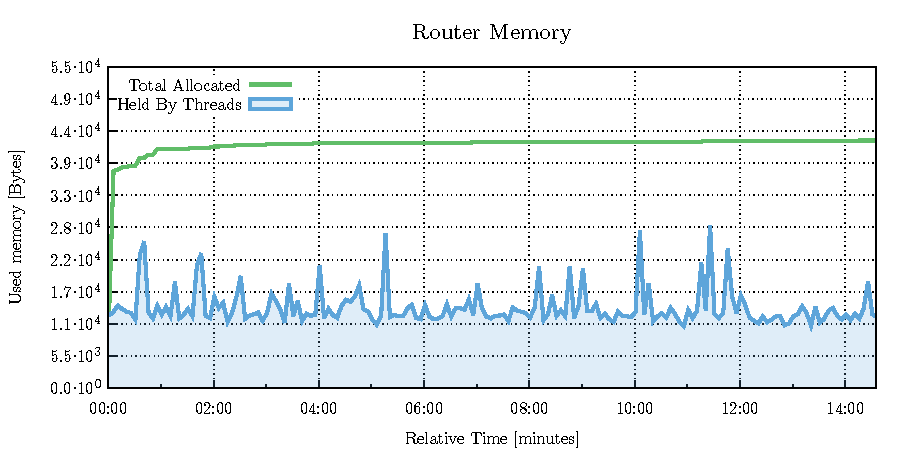
\includegraphics[width=1\linewidth]{obrazky-figures/charts/singlepoint-router-throughput-memory.pdf}
	\caption{The total allocated memory and memory-in-use by Qpid-Dispatch during the test. The data were collected by the inspector every 5\,seconds.}
	\label{fig:router-single-memory}
\end{figure}

\begin{figure}[H]
	\centering
	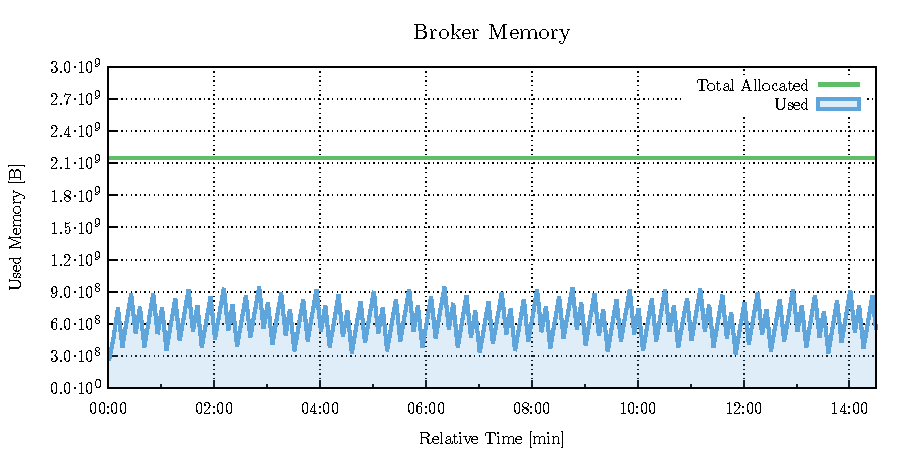
\includegraphics[width=1\linewidth]{obrazky-figures/charts/singlepoint-broker-throughput-memory.pdf}
	\caption{The total memory allocation for the Broker service. One can see that the broker allocates more memory compared to Qpid-Dispatch in the Figure \ref{fig:router-single-memory}.}
	\label{fig:broker-single-memory}
\end{figure}


\subsubsection*{Multipoint Topology}
For the multipoint experiments we used topologies depicted in the Figures \ref{fig:basic_topology_router_line} and \ref{fig:basic_topology_broker_line}. The network throughput can naturally be influenced by other device connected to the topology. So the singlepoint topology was extended by another components by adding two other routers around the original SUT. The versions of the newly added SUTs are the same as the original ones.

\begin{figure}[H]
	\centering
	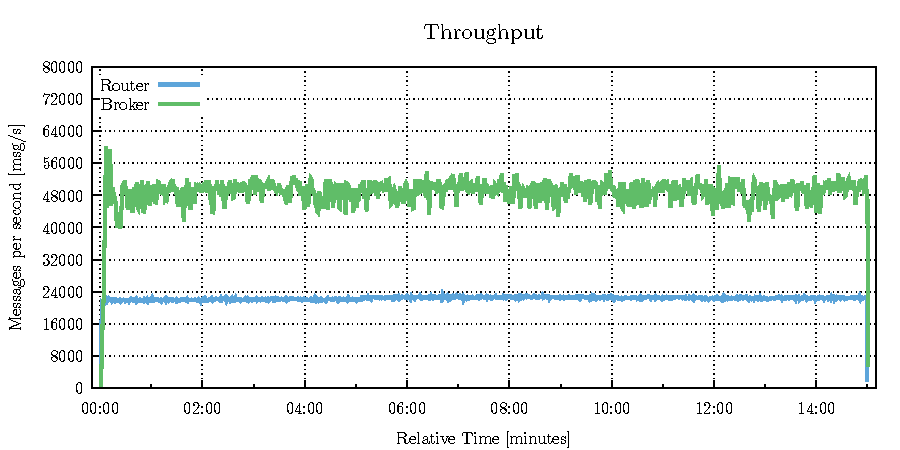
\includegraphics[width=1\linewidth]{obrazky-figures/charts/multipoint-throughput.pdf}
	\caption{Measured throughput of Qpid-Dispatch and Message Broker during the multipoint case study. One can see the performance degradation of Qpid-Dispatch and improvements of Message Broker on that Figure.}
	\label{fig:rate-multipoint-router}
\end{figure}

In the Figure \ref{fig:rate-multipoint-router} one can see, that adding routers to the broker node raises achievable throughput to the 48\,000 messages per second. On the other hand, the topology consisting only of the routers shows significant performance degradation. The throughput falls from the 90\,000 messages per second to the approximately 23\,000 messages per second. This degradation is caused by the interior flow-control mechanism, which should prevent the overload of the network. However, in this case study we can see that the performance degradation is too high and the mechanism used in the Qpid-Dispatch should be re-implemented.


\begin{figure}[H]
	\centering
	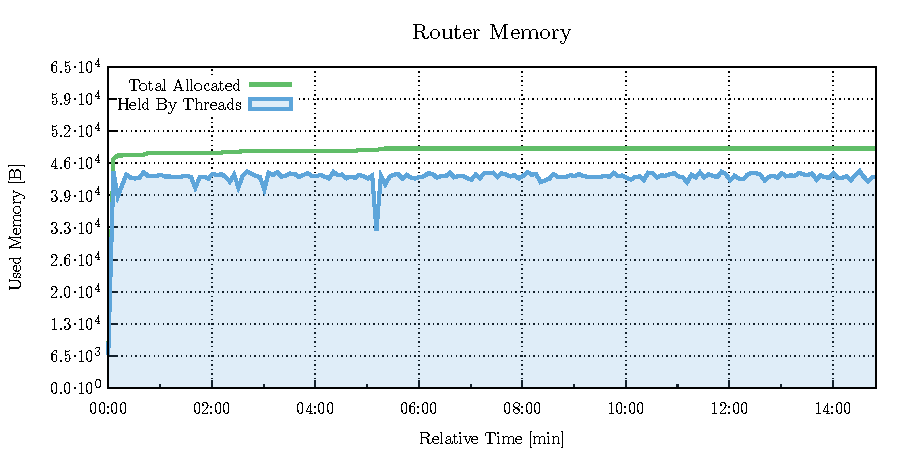
\includegraphics[width=1\linewidth]{obrazky-figures/charts/multipoint-router-only-throughput-memory.pdf}
	\caption{Qpid-Dispatch's memory usage during the multipoint case study. Used memory is higher than in the single-point.}
	\label{fig:router-multipoint-memory}
\end{figure}

Based on that mechanism, the memory usage of the middle router depicted in the Figure \ref{fig:router-multipoint-memory} is higher than during the previous case study. Memory used by all threads is around two times higher and the mean value is around 43\,kB. On the other hand, the memory allocated for the broker component remains the same as in the previous case study. The memory monitoring for this case study is depicted in the Figure \ref{fig:broker-multipoint-memory}.

\begin{figure}[H]
	\centering
	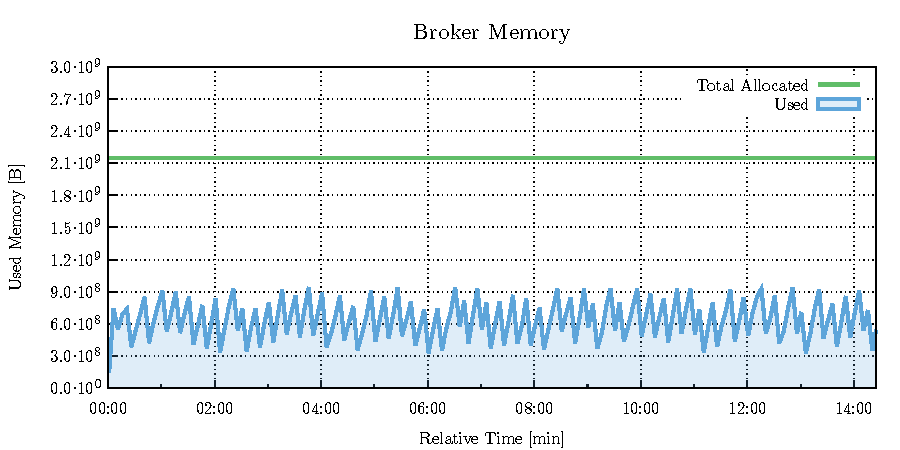
\includegraphics[width=1\linewidth]{obrazky-figures/charts/multipoint-router-broker-throughput-memory.pdf}
	\caption{Memory usage for Broker remains almost the same as in the single-point case, but with less spikes.}
	\label{fig:broker-multipoint-memory}
\end{figure}


\subsubsection*{Conclusion}
The collected data during the throughput measurements reveal unexpected and considerable performance degradation in the serial connection of the Qpid-Dispatch. The comparison between the single and multi-point case study is in the Figure \ref{fig:basic-throughput-comparison}, which groups together all throughput measurements data into one chart. Here one can see the performance improvement between single instance Broker test and the test of topology with the broker (yellow and green color), and performance degradation between router topologies (red and blue color). The summary of results is also available in the Table \ref{tab:throughput-summary}.

% Please add the following required packages to your document preamble:
% \usepackage{multirow}
% \usepackage[table,xcdraw]{xcolor}
% If you use beamer only pass "xcolor=table" option, i.e. \documentclass[xcolor=table]{beamer}
\begingroup
\setlength{\tabcolsep}{10pt} % Default value: 6pt
\renewcommand{\arraystretch}{1.35} % Default value: 1
	\begin{table}[h]
	\centering
	\caption{Table with collected data with highlighted performance improvements and degradations.}
	\label{tab:throughput-summary}
	\begin{tabular}{|l|r|r|r|r|}
	\hline
	\rowcolor[HTML]{C5E3DF}
	\cellcolor[HTML]{C5E3DF} & \multicolumn{2}{c|}{\cellcolor[HTML]{C5E3DF}\textbf{Throughput (Msg/s)}} & \multicolumn{2}{c|}{\cellcolor[HTML]{C5E3DF}\textbf{Memory}} \\ \cline{2-5}
	\rowcolor[HTML]{C5E3DF}
	\multirow{-2}{*}{\cellcolor[HTML]{C5E3DF}\textbf{Test Type}} & \textbf{Expected} & \textbf{Measured} & \textbf{Total} & \textbf{Used max} \\ \hline
	\textbf{Single Router} & - & 90\,000 & 45\,kB & 28\,kB \\ \hline
	\textbf{Single Broker} & - & 30\,000 & 2\,GB & 0.9\,GB \\ \hline
	\textbf{Line of Routers} & 90\,000 & \cellcolor[HTML]{FFCCC9}23\,000 & 49\,kB & 43\,kB \\ \hline
	\textbf{Line with Broker} & 30\,000 & \cellcolor[HTML]{9AFF99}48\,000 & 2\,GB & 0.9\,GB \\ \hline
	\end{tabular}
	\end{table}
\endgroup

\begin{figure}[H]
	\centering
	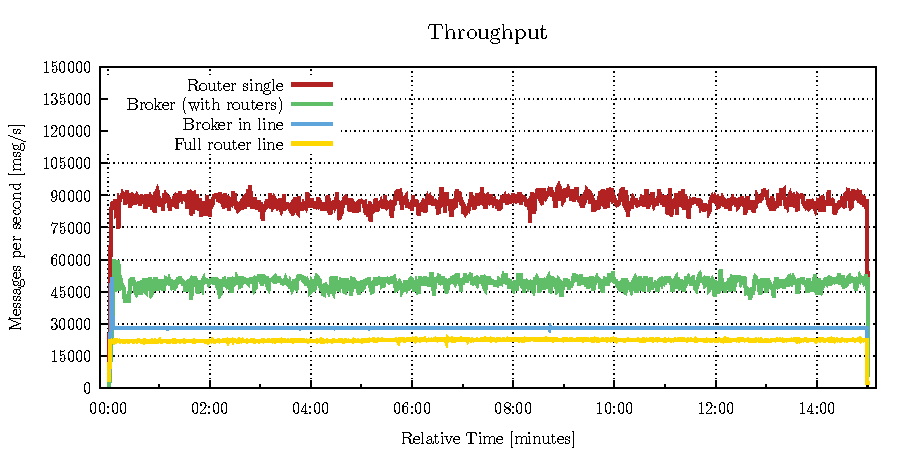
\includegraphics[width=1\linewidth]{obrazky-figures/charts/basic-throughput.pdf}
	\caption{The comparison of all measured throughputs for different components and topologies.}
	\label{fig:basic-throughput-comparison}
\end{figure}


\subsection{Latency}
\label{Latency}
Latency is measured only by Maestro Receiver from certain load samples. Since the Broker is a distribution service, which needs to store messages for some time, or create and keep queues for clients, it has higher requirements for system resources. On the other hand Qpid-dispatch has only one purpose\,---\,to route the messages. This makes it more faster than the Broker. So high load can be unprofitable if one wants better latency during the communication, especially in the case of topology with the broker. The broker can handle less messages than router, but using router can raise broker's throughput since it can control the load. Thus it gives more time to broker to process messages even with higher load. The test cases for latency measurements has slightly different settings than throughput measurement. The settings for this measurements are shown in the Table \ref{tab:test_case_latency}. Note, that \emph{RATE} and \emph{TEST\_DURATION} are sets for each of five connected clients, which means that test is finished after sending 10\,000\,000 messages.

% Please add the following required packages to your document preamble:
% \usepackage{multirow}
% \usepackage[table,xcdraw]{xcolor}
% If you use beamer only pass "xcolor=table" option, i.e. \documentclass[xcolor=table]{beamer}
\begingroup
\setlength{\tabcolsep}{10pt} % Default value: 6pt
\renewcommand{\arraystretch}{1.35} % Default value: 1
	\begin{table}[H]
	\centering
	\caption{Test case settings for latency measurements.}
	\label{tab:test_case_latency}
	\begin{tabular}{|l|r|r|r|r|}
	\hline
	\rowcolor[HTML]{C5E3DF}
	\cellcolor[HTML]{C5E3DF} & \multicolumn{4}{c|}{\cellcolor[HTML]{C5E3DF}\textbf{Value}} \\ \cline{2-5}
	\rowcolor[HTML]{C5E3DF}
	\cellcolor[HTML]{C5E3DF} & \multicolumn{2}{c|}{\cellcolor[HTML]{C5E3DF}\textbf{Singlepoint}} & \multicolumn{2}{c|}{\cellcolor[HTML]{C5E3DF}\textbf{Multipoint}} \\ \cline{2-5}
	\rowcolor[HTML]{C5E3DF}
	\multirow{-3}{*}{\cellcolor[HTML]{C5E3DF}\textbf{Test Property}} & \textbf{Router} & \textbf{Broker} & \textbf{Full Router} & \textbf{With Broker} \\ \hline
	\textbf{MESSAGE\_SIZE [B]} & \multicolumn{4}{r|}{256} \\ \hline
	\textbf{PARALLEL\_COUNT} & \multicolumn{4}{r|}{5} \\ \hline
	\textbf{TEST\_DURATION} & \multicolumn{4}{r|}{2\,000\,000 messages} \\ \hline
	\textbf{RATE} & 15\,000 & 4\,600 & 3\,600 & 7\,600 \\ \hline
	\end{tabular}
	\end{table}
\endgroup

\subsubsection*{Single Node}
The latency measurements are done with 80\% of maximum rate, which were discussed in the Subsection \ref{Throughput}. In the Figure \ref{fig:latency-single-router} you can see the latency difference that we measured between Qpid-Dispatch and Message Broker. In single node measurements, the router's latency is slightly higher in the most of the cases. After discussion we did not find a reason why is router slower then Broker in that case.

%This is caused by the Maestro Sender and Receiver technologies, because they are implemented in Java and Maestro Sender and Receiver are using JMS for sending and receiving messages, which is same approach as the Broker uses. For better latency comparison it is necessary to measure Broker's latency with current implementations and Qpid-Dispatch's latency with Python clients. However, the current version of Maestro offers only the JMS clients.

\begin{figure}[H]
	\centering
	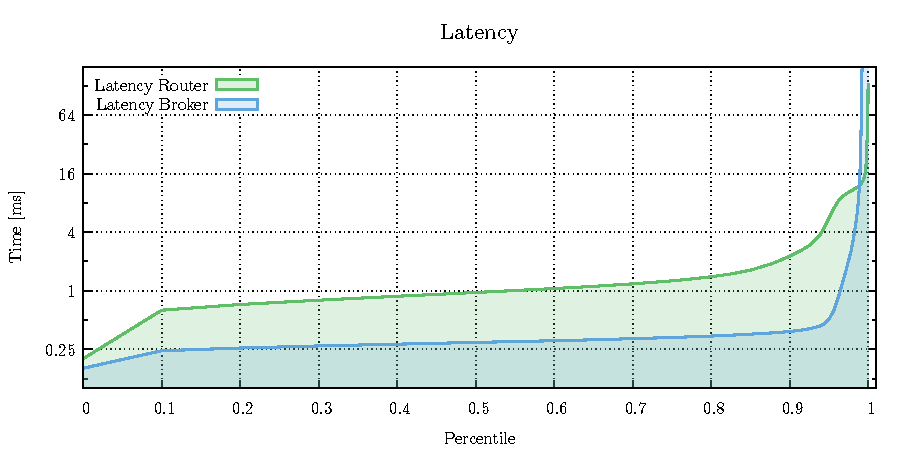
\includegraphics[width=1\linewidth]{obrazky-figures/charts/singlepoint-latency.pdf}
	\caption{Latency chart showing the difference between the router and the broker latency at 80\,\% of maximum rate.}
	\label{fig:latency-single-router}
\end{figure}

\begin{figure}[H]
	\centering
	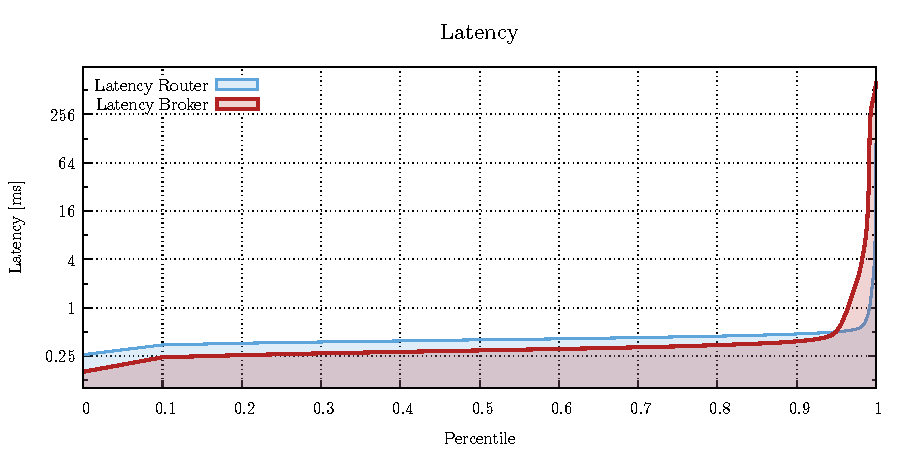
\includegraphics[width=1\linewidth]{obrazky-figures/charts/singlepoint-latency-18k.pdf}
	\caption{Latency chart showing the difference between the router and the broker latency at same load. Router's latency is significantly better then in previous case.}
	\label{fig:latency-single-same-load}
\end{figure}

Then we tried to rerun the latency measurements with same load for both test cases. The load was set to 4\,500 messages per second for each connected client. The output is depicted in the Figure \ref{fig:latency-single-same-load}, where the router is significantly faster, but still slower than Broker. This is probably caused by some Maestro internal processes.

The memory used by Qpid-dispatch is slightly lower and much stable than in the case of maximum throughput as one can see in the Figure \ref{fig:latency-single-router-memory}. This proves, that used memory is dependent on the load. If the load on the router is higher then it needs more memory for proper routing.

\begin{figure}[H]
	\centering
	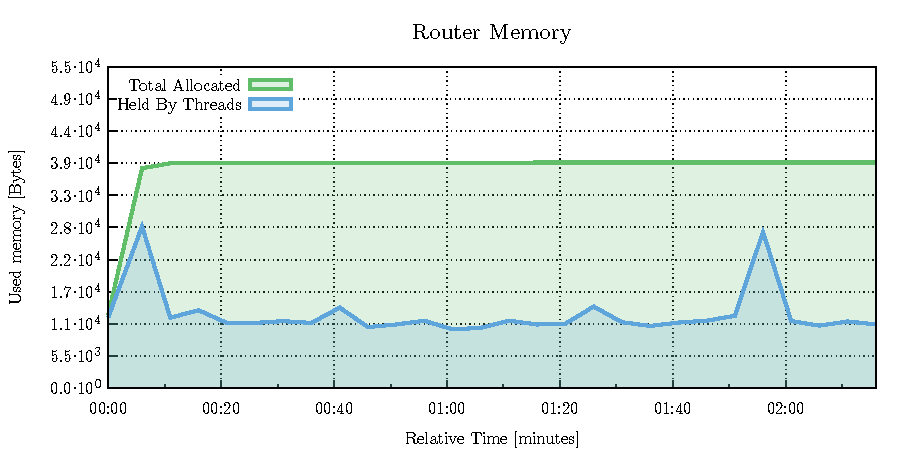
\includegraphics[width=1\linewidth]{obrazky-figures/charts/singlepoint-router-latency-memory.pdf}
	\caption{Memory usage of Qpid-Dispatch is much stable when the router is not under the maximum load. The spikes are caused by some unexpected events in the topology.}
	\label{fig:latency-single-router-memory}
\end{figure}


\begin{figure}[H]
	\centering
	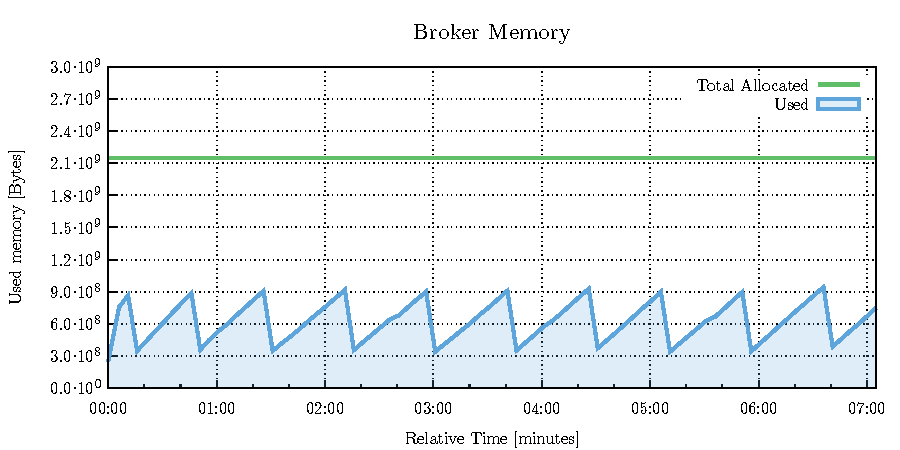
\includegraphics[width=1\linewidth]{obrazky-figures/charts/singlepoint-broker-latency-memory.pdf}
	\caption{The Broker's memory usage has lesser spike when the load is only about of 80\,\% of maximum.}
	\label{fig:latency-single-broker-memory}
\end{figure}

In the Figure \ref{fig:latency-single-broker-memory} one can see the Inspector output for Broker's used memory. The used memory here is much stable than in the previous cases, which is caused, as in the router case, by lower load on the Broker. Maximum used memory stags the same as in the previous cases.

\subsubsection*{Multipoint Topology}
One can see the measured latency on multinode topology of three routers, and two routers with middle-broker in the Figure \ref{fig:latency-multipoint-router}. The latency curve proves, that routers are able to deliver messages into its destination faster than the topology with the Broker, again because the Broker needs to store them in the memory. The latency of the topology with broker reaches around 16\,$\mu$s in 90\,\% of samples; on the other hand, topology consisting of routers has significantly better latency that is around 1\,$\mu$s in 90\,\% of samples. The conclusion is that the collected data proves the router should be much faster than the broker during the certain circumstances..

\begin{figure}[H]
	\centering
	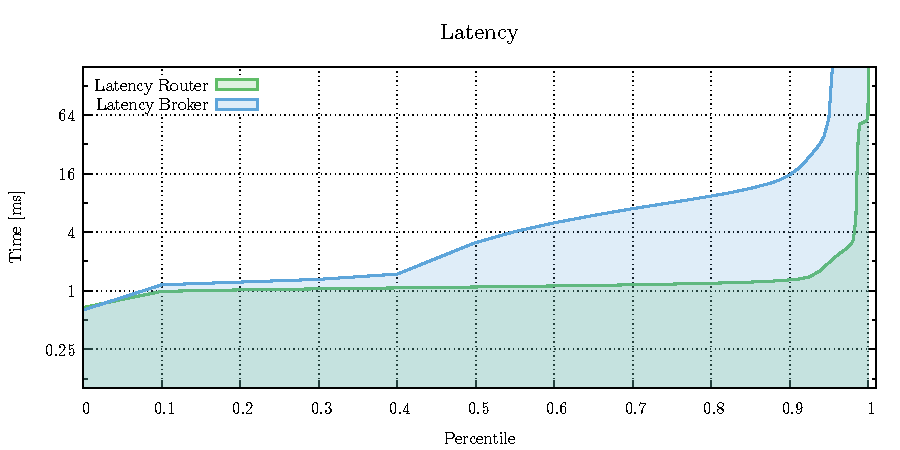
\includegraphics[width=1\linewidth]{obrazky-figures/charts/multipoint-latency.pdf}
	\caption{Latency comparison between topologies with only routers and with the middle-broker. The router network is here significantly faster.}
	\label{fig:latency-multipoint-router}
\end{figure}

\begin{figure}[H]
	\centering
	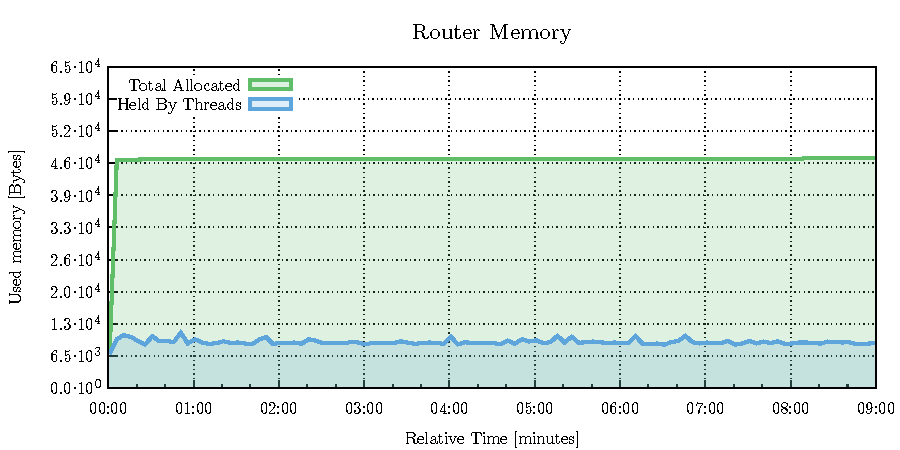
\includegraphics[width=1\linewidth]{obrazky-figures/charts/multipoint-router-only-latency-memory.pdf}
	\caption{Memory usage shows, that memory usage of the router is affected by the throughput.}
	\label{fig:latency-multiple-router-memory}
\end{figure}

Collected data about the memory usage proves the previous statements. In the Figure \ref{fig:latency-multiple-router-memory} we show used memory by Qpid-Dispatch. The curve is very stable and the values moves around the 9\,MB of used memory. The used memory by the Broker is shown in the Figure \ref{fig:latency-multiple-broker-memory} and is very similar as in the previous measurements.

\begin{figure}[H]
	\centering
	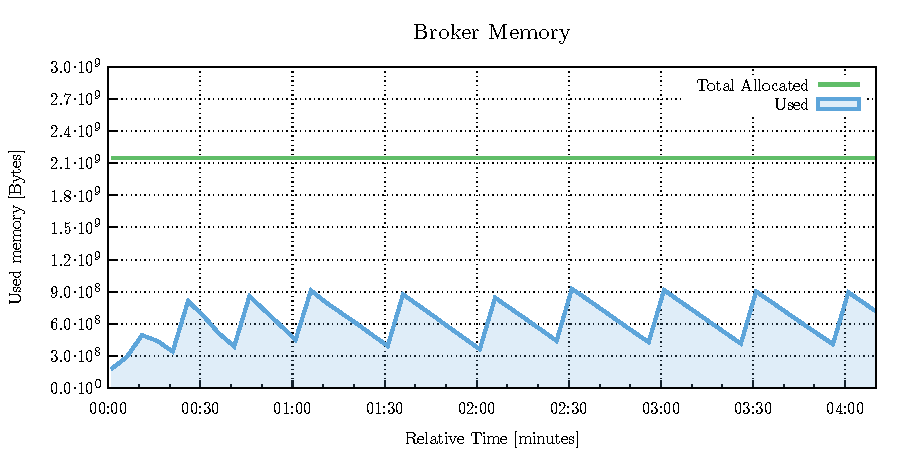
\includegraphics[width=1\linewidth]{obrazky-figures/charts/multipoint-router-broker-latency-memory.pdf}
	\caption{Chart of memory allocation on the Broker node..}
	\label{fig:latency-multiple-broker-memory}
\end{figure}

\subsubsection*{Conclusion}
During the latency measurements we collected and compared data for the Qpid-Dispatch and Message Broker topologies. The summa
ry of latency measurements is available in the Table \ref{tab:latency-summary}. Is it was already mentioned, Qpid-Dispatch is faster in the model environment the Message Broker.

% Please add the following required packages to your document preamble:
% \usepackage{multirow}
% \usepackage[table,xcdraw]{xcolor}
% If you use beamer only pass "xcolor=table" option, i.e. \documentclass[xcolor=table]{beamer}
\begingroup
\setlength{\tabcolsep}{10pt} % Default value: 6pt
\renewcommand{\arraystretch}{1.35} % Default value: 1
	\begin{table}[H]
	\centering
	\caption{The summary table with collected latency data with highlighted performance improvements and degradations.}
	\label{tab:latency-summary}
	\begin{tabular}{|l|r|r|r|r|r|}
	\hline
	\rowcolor[HTML]{C5E3DF}
	\multicolumn{1}{|c|}{\cellcolor[HTML]{C5E3DF}} & \multicolumn{2}{c|}{\cellcolor[HTML]{C5E3DF}\textbf{Latency ($\mu$s)}} & \multicolumn{2}{c|}{\cellcolor[HTML]{C5E3DF}\textbf{Memory}} & \multicolumn{1}{c|}{\cellcolor[HTML]{C5E3DF}} \\ \cline{2-5}
	\rowcolor[HTML]{C5E3DF}
	\multicolumn{1}{|c|}{\multirow{-2}{*}{\cellcolor[HTML]{C5E3DF}\textbf{Test Type}}} & \multicolumn{1}{c|}{\cellcolor[HTML]{C5E3DF}\textbf{90 \%}} & \multicolumn{1}{c|}{\cellcolor[HTML]{C5E3DF}\textbf{99 \%}} & \multicolumn{1}{c|}{\cellcolor[HTML]{C5E3DF}\textbf{Total}} & \multicolumn{1}{c|}{\cellcolor[HTML]{C5E3DF}\textbf{Used max}} & \multicolumn{1}{c|}{\multirow{-2}{*}{\cellcolor[HTML]{C5E3DF}\textbf{\begin{tabular}[c]{@{}c@{}}Duration \\ (s)\end{tabular}}}} \\ \hline
	\textbf{Single Router} & 2.263 & 12.495 & 38 KB & 28 KB & \cellcolor[HTML]{9AFF99}136 \\ \hline
	\textbf{Single Broker} & 0.386 & 181.759 & 2 GB & 0.9 GB & \cellcolor[HTML]{FFCCC9}425 \\ \hline
	\textbf{Line of Routers} & \cellcolor[HTML]{9AFF99}1.292 & 50.815 & 46 KB & 8 KB & \cellcolor[HTML]{FFCCC9}540 \\ \hline
	\textbf{Line with Broker} & \cellcolor[HTML]{FFCCC9}15.487 & 1031.167 & 2 GB & 0.9 GB & \cellcolor[HTML]{9AFF99}250 \\ \hline
	\end{tabular}
	\end{table}
\endgroup


\section{Behavior Measurements}
\label{Behavior Measurements}
Moreover, we present some results collected during the behavioral testing using the Maestro Agent extension. The topologies used in the following scenarios are depicted in the Figure \ref{fig:agent_topologies}. The topology depicted in the Figure \ref{fig:agent_line} is used to demonstrate Agent functions and message loss during the crash. The other topology depicted in the Figure \ref{fig:agent_redundant} represent a basic line link with redundant router\,2 which is configured as a slave and root router\,3 which is configured as a master. Here we demonstrate the recovery time of Qpid-Dispatch.

\begin{figure}[h]
	\centering
	\begin{minipage}{0.45\linewidth}
		\subfloat[Line topology with connected Inspector and Agent.\label{fig:agent_line}]{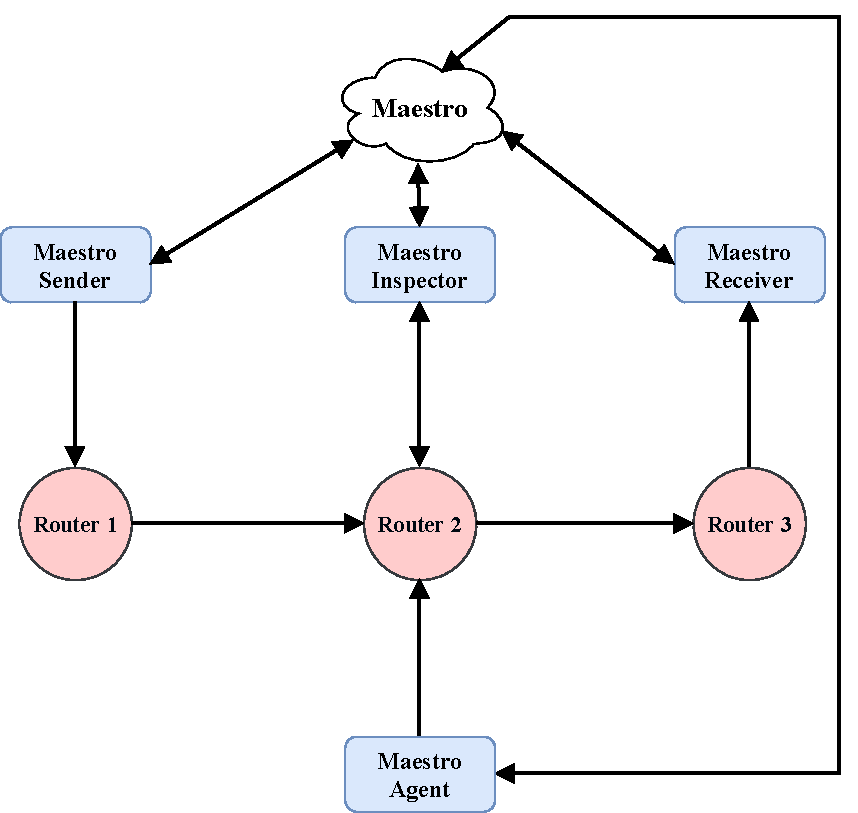
\includegraphics[width=\linewidth]{obrazky-figures/basic_topology_router_agent_line.pdf}}
	\end{minipage}
	\begin{minipage}{0.45\linewidth}
		\subfloat[Topology with redundant router.\label{fig:agent_redundant}]{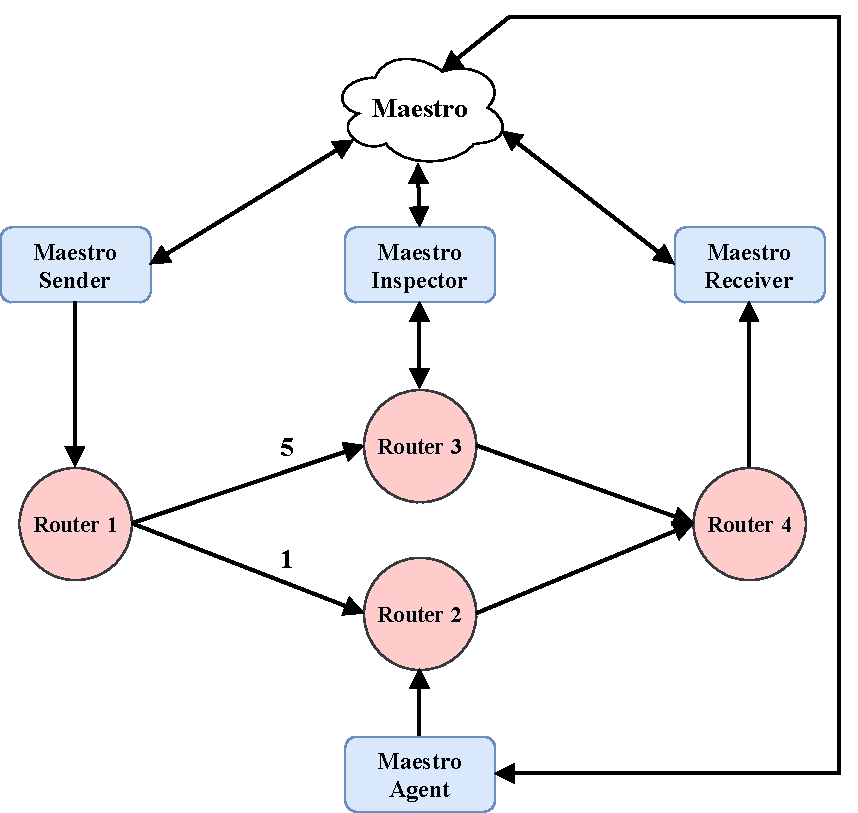
\includegraphics[width=\linewidth]{obrazky-figures/basic_topology_router_agent_redundant.pdf}}
	\end{minipage}
	\caption[Examples of experimental topologies created for behavioral performance testing and experiments with Maestro.]{Examples of experimental topologies created for behavioral performance testing and experiments with Maestro. The arrows indicate the communication path between topology components and the numbers represent the cost for the path.}\label{fig:agent_topologies}
\end{figure}

On each topology we performed four tests with different actions executed by the Agent. The test properties remains the same as during the latency testing for router line topology with the difference in test duration, which was set to 1\,500\,000 messages per connected client. The following actions, with additional parameter such as duration, were performed during the test:

\begin{itemize}
	\setlength\itemsep{0em}
	\item \textbf{Restart}\,---\,simple router restart.
	\item \textbf{Shutdown}\,---\,simple shutdown and restart for different time duration.
\end{itemize}

\subsection{Agent Demonstration}
\label{Agent Demonstration}
The agent performed specific action in the third minute of the test scenario (there can be a small delay caused by the repository download on the Agent). The shutdown actions have specific duration, which was set to 10, 60 and 120 seconds. Since the topology used for this type of tests does not have any redundant path to destination or Broker work message store, the messages got lost during the actions. Note, that the test was triggered without message acknowledgment settings for the router and the clients. In the Figure \ref{fig:agent-throughput} one can see the throughput affected by the restart and shutdown actions in every case study. The magnitude of the action impact is based on the action duration, hence, the longer shutdown will lose more message than short restart. However, the chart proves, that routers can establish lost connection with the clients without problems when the router is started again. The different test duration points to the fact, that Maestro detect connections issues and wait for the connection establishment.

\begin{figure}[H]
	\centering
	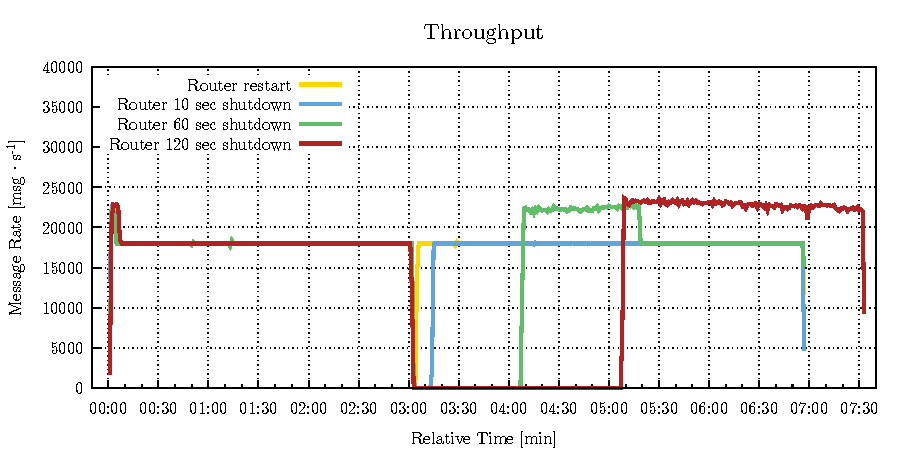
\includegraphics[width=1\linewidth]{obrazky-figures/charts/agent-throughput.pdf}
	\caption{Maestro Agent demonstration against a simple topology with restart and shutdown in the third minute of test.}
	\label{fig:agent-throughput}
\end{figure}

The latency is affected as well, one can see that significant message amount raises the latency from 1\,$\mu$s to 64\,$\mu$s. However note, that some messages were lost which lead to smaller number of samples for latency computation. The message lost ratio is captured in the Table~\ref{tab:agent_demonstration}. One can see that Qpid-Dispatch lost 39\,518 messages which correspond to throughput for 2\,195\,$\mu$s. Regarding this, we can say that router restart interrupt the link for 2,195\,$\mu$s.

\begin{figure}[H]
	\centering
	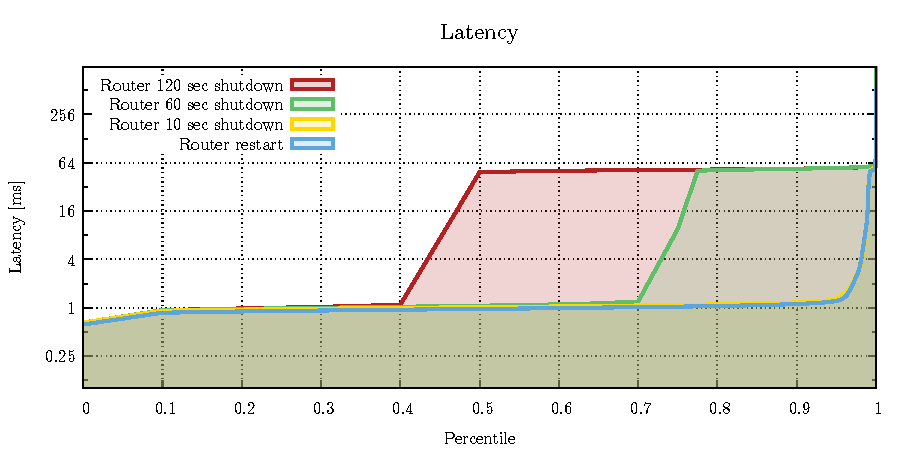
\includegraphics[width=1\linewidth]{obrazky-figures/charts/agent-latency.pdf}
	\caption{Latency diagram affected by the actions simulating the connection issues.}
	\label{fig:agent-latency}
\end{figure}

% Please add the following required packages to your document preamble:
% \usepackage{multirow}
% \usepackage[table,xcdraw]{xcolor}
% If you use beamer only pass "xcolor=table" option, i.e. \documentclass[xcolor=table]{beamer}
\begingroup
\setlength{\tabcolsep}{10pt} % Default value: 6pt
\renewcommand{\arraystretch}{1.35} % Default value: 1
	\begin{table}[H]
	\centering
	\caption{Table with summary of lost messages during the specific actions on the middle router node.}
	\label{tab:agent_demonstration}
	\begin{tabular}{|l|r|r|r|r|}
	\hline
	\rowcolor[HTML]{C5E3DF}
	\cellcolor[HTML]{C5E3DF} & \multicolumn{1}{c|}{\cellcolor[HTML]{C5E3DF}} & \multicolumn{3}{c|}{\cellcolor[HTML]{C5E3DF}\textbf{Message Lost}} \\ \cline{3-5}
	\rowcolor[HTML]{C5E3DF}
	\multirow{-2}{*}{\cellcolor[HTML]{C5E3DF}\textbf{Action}} & \multicolumn{1}{c|}{\multirow{-2}{*}{\cellcolor[HTML]{C5E3DF}\textbf{Duration (s)}}} & \multicolumn{1}{l|}{\cellcolor[HTML]{C5E3DF}\textbf{Expected}} & \multicolumn{1}{l|}{\cellcolor[HTML]{C5E3DF}\textbf{Lost}} & \multicolumn{1}{l|}{\cellcolor[HTML]{C5E3DF}\textbf{Percent}} \\ \hline
	Restart & 0 & & 39\,518 & 0.53 \% \\ \cline{1-2} \cline{4-5}
	 & 10 & & 220\,445 & 2.94 \% \\ \cline{2-2} \cline{4-5}
	 & 60 & & 871\,661 & 11,62 \% \\ \cline{2-2} \cline{4-5}
	\multirow{-3}{*}{Shutdown} & 120 & \multirow{-4}{*}{7\,500\,000} & 918\,266 & 12.25 \% \\ \hline
	\end{tabular}
	\end{table}
\endgroup


\subsection{Measurement With Redundant Router}
During this experiment the Agent performs the same actions as in the previous test cases. The difference is, that given topology now has a slave router connected into the network which is ready to route the messages when master router crash. In the Figure \ref{fig:agent-redundant-throughput} is depicted the throughput for all tests on this topology. The Agent performs actions in third minute which causes spike under the stable load curve, but the throughput is raised back quickly. This spike is caused by a small delay when the redundant router starts his job. It needs some time for warm-up, which involves the memory allocation depicted in the Figure \ref{fig:agent-redundant-memory}. As one can see, there is no additional spikes after then master is turned up, hence the first spike is cause only by first routing redundant router.

\begin{figure}[H]
	\centering
	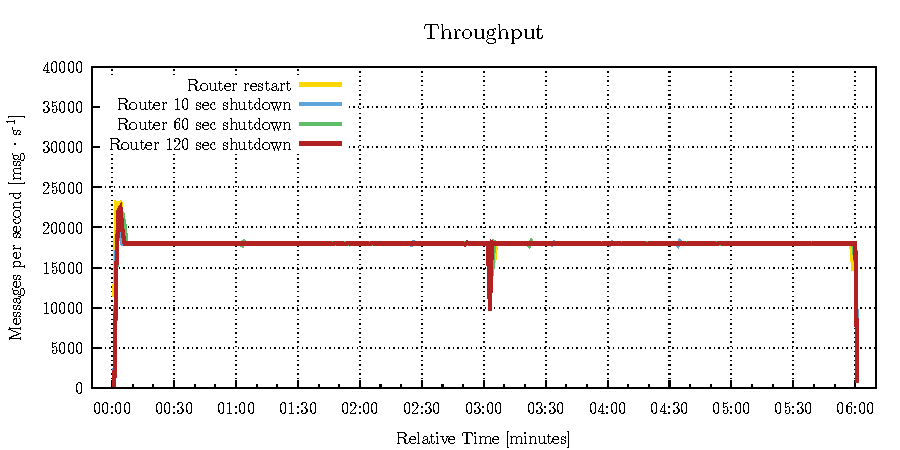
\includegraphics[width=1\linewidth]{obrazky-figures/charts/agent-redundant-throughput.pdf}
	\caption{Throughput comparison between the test cases with different Agent executions. The spike is caused by warm-up period of redundant router.}
	\label{fig:agent-redundant-throughput}
\end{figure}

\begin{figure}[H]
	\centering
	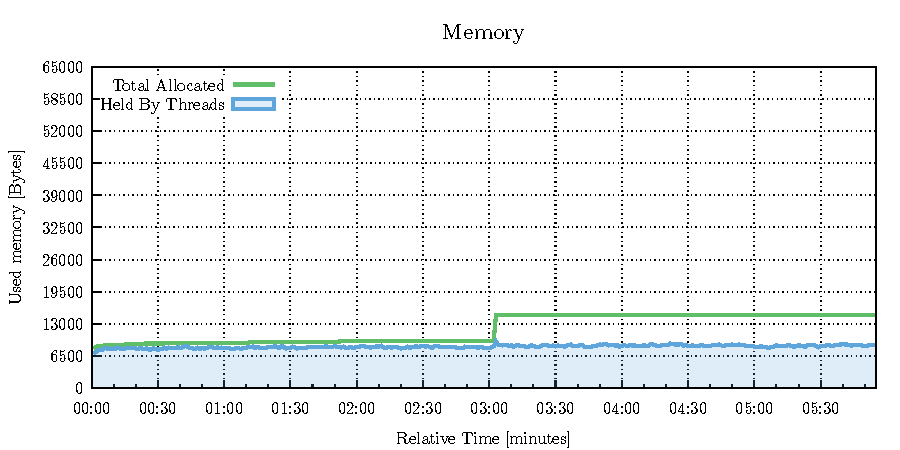
\includegraphics[width=1\linewidth]{obrazky-figures/charts/restart-redundant-agent-memory.pdf}
	\caption{Allocated memory for redundant router during the restart. One can see that router allocated new memory when the master router crashed and the slave had to handle the load. This memory is allocated until the tear down.}
	\label{fig:agent-redundant-memory}
\end{figure}

\begin{figure}[H]
	\centering
	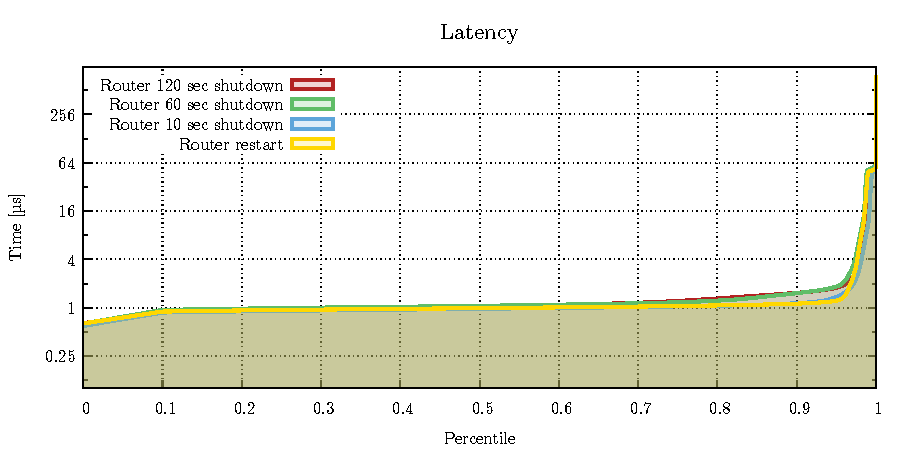
\includegraphics[width=1\linewidth]{obrazky-figures/charts/agent-redundant-latency.pdf}
	\caption{Latency diagram with Agent actions and redundant router in the topology. The latency remains the same for all the test cases which points to a good routing between the routers.}
	\label{fig:agent-redundant-latency}
\end{figure}

Since we want to know how long it takes to router to re-establish connections after the crash we can find the answer in the Figure \ref{fig:agent-redundant-unpressetled}. One can see the detail of test case with restart router action which is executed three minutes after the test starts. The monitored router is the redundant one, so we can see that it handled the load for two seconds. After this time the master router was able to route load again and the slave router just waits for another communication. This statement is also supported by results collected and discuss in the Section \ref{Agent Demonstration}.

\begin{figure}[H]
	\centering
	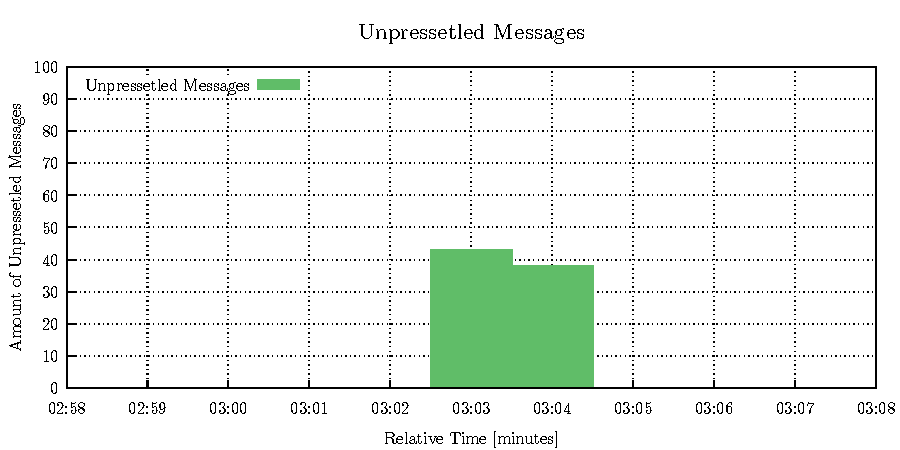
\includegraphics[width=1\linewidth]{obrazky-figures/charts/restart-redundant-agent-routerLink.pdf}
	\caption{Chart captures unsettled messages on the redundant router node. The slave router handled load for two seconds.}
	\label{fig:agent-redundant-unpressetled}
\end{figure}

The conclusion is, that Qpid-Dispatch is able to recover after a crash in less than three seconds, when there is no block for service start. When the router is down, the topology is updated and the previous hop does not have path to the crashed router, so the clients cannot affect the router start after the crash. However, even with redundant path there is a chance that some messages are lost as it is captured in the Table \ref{tab:agent_redundant_lost}. For avoid this cases it is necessary to turn on acknowledge mechanism for AMQP messages, which should avoid message lost but it will affect the performance.

% Please add the following required packages to your document preamble:
% \usepackage{multirow}
% \usepackage[table,xcdraw]{xcolor}
% If you use beamer only pass "xcolor=table" option, i.e. \documentclass[xcolor=table]{beamer}
\begingroup
\setlength{\tabcolsep}{10pt} % Default value: 6pt
\renewcommand{\arraystretch}{1.35} % Default value: 1
	\begin{table}[H]
	\centering
	\caption{Table with summary of lost messages during the perform specific action on the middle router node without redundant path.}
	\label{tab:agent_redundant_lost}
	\begin{tabular}{|l|r|r|r|r|}
	\hline
	\rowcolor[HTML]{C5E3DF}
	\cellcolor[HTML]{C5E3DF} & \multicolumn{1}{c|}{\cellcolor[HTML]{C5E3DF}} & \multicolumn{3}{c|}{\cellcolor[HTML]{C5E3DF}\textbf{Message Lost}} \\ \cline{3-5}
	\rowcolor[HTML]{C5E3DF}
	\multirow{-2}{*}{\cellcolor[HTML]{C5E3DF}\textbf{Action}} & \multicolumn{1}{c|}{\multirow{-2}{*}{\cellcolor[HTML]{C5E3DF}\textbf{Duration (s)}}} & \multicolumn{1}{l|}{\cellcolor[HTML]{C5E3DF}\textbf{Expected}} & \multicolumn{1}{l|}{\cellcolor[HTML]{C5E3DF}\textbf{Lost}} & \multicolumn{1}{l|}{\cellcolor[HTML]{C5E3DF}\textbf{Percent}} \\ \hline
	Restart & 0 & & 21\,804 & 0.29 \% \\ \cline{1-2} \cline{4-5}
	 & 10 & & 13\,359 & 0.18 \% \\ \cline{2-2} \cline{4-5}
	 & 60 & & 16\,205 & 0.22 \% \\ \cline{2-2} \cline{4-5}
	\multirow{-3}{*}{Shutdown} & 120 & \multirow{-4}{*}{7\,500\,000} & 22\,042 & 0.29 \% \\ \hline
	\end{tabular}
	\end{table}
\endgroup
